
\centerline{\textbf{ \LARGE Interupts, System calls, CPU Modes}}


% ----------------------------------------------------------------------------


  \begin{enumerate}

  \item CPU Instructions - privileged and non-privileged.
  \begin{figure}[h]
      \centering   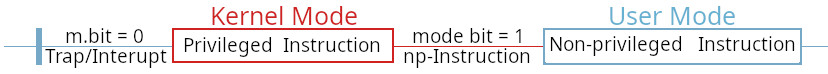
\includegraphics[scale=2.5]{./images/cpu_mode_03.jpeg}
  \end{figure}
  \item CPU Dual mode - User Mode and Kernel Mode.
  \begin{enumerate}
        \item In above figure.
        \item Interupts/Traps cause CPU to change mode from user(1) to kernel(0) mode.
        \item System executes privileged instructions.
        \item A non-privileged instruction which do not cause interupt changes kernel(0) mode to user(1) mode.
        \item Dual Mode ensures protection and security from unauthorized users.
  \end{enumerate}


  \item Privileged Instruction.
  \begin{enumerate}
        \item Privileged instructions executed only in Kernel Mode.
        \item Ex programs : kernel code, schedular, interupt service routine, drivers, code to access hardware.
        \item Provides unrestricted access to
         \begin{enumerate}
            \item the system resources
            \item hardware
            \item low-level system operations(ex. setting up memory mappings).
          \end{enumerate}
        \item Executing privileged instruction in user mode is illegal. Hardware traps it in the OS.
        \item Privileged Instruction can modify the contents of the Timer.
  \end{enumerate}

  \item Non-Privileged Instruction.
  \begin{enumerate}
        \item Executed only in User Mode.
        \item Provide general purpose computing.
        \item Ensures that user processes do interfere.
        \item Provides access to user-level resources such as files and memory.
  \end{enumerate}


  \item Interupts, Interrupt Vector Table and Interrupt Service Routine(interrupt handler)
  \begin{enumerate}
        \item Types - Hardware Interupts and Software Interupts.
        \item Every interrupt has IS-Routine.
        \item IVT holds address of IS-Routine for each interupt.
        \item IS-Routine is part of Kernal. (Check this point)
  \end{enumerate}{enumerate}


  \item Software Interupts
  \begin{enumerate}
        \item Traps and Exceptions.
        \item Software Interrupts serve as a signal for the OS to carry out a certain function or respond to an error condition.
        \item When a process executes an “Interrupt instruction” a software interrupt is generated.
  \end{enumerate}

  \begin{figure}[h]
      \centering   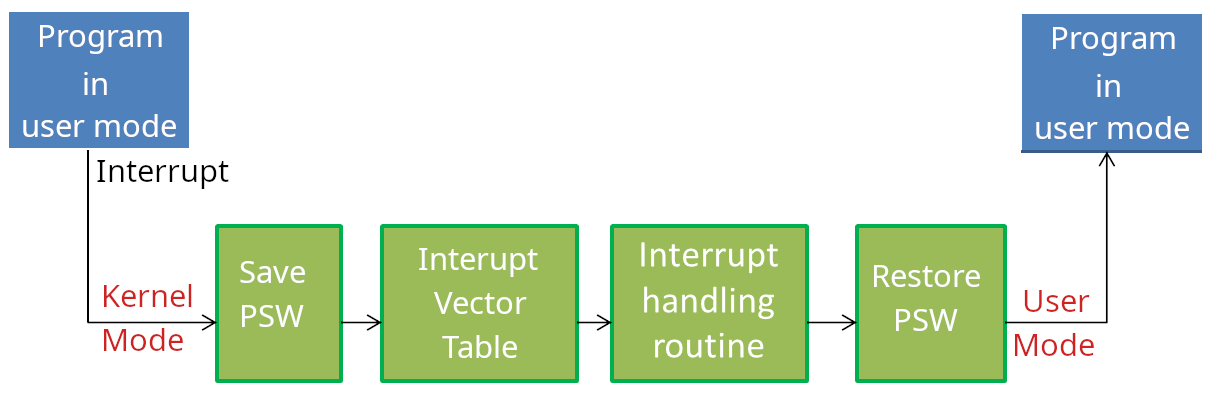
\includegraphics[scale=1.6]{./images/Interupt_01.jpeg}
  \end{figure}

  \begin{minipage}{\linewidth}
  \item Interupt flow.
  \begin{enumerate}
        \item CPU finishes executing current execution cycle.
        \item CPU checks for interupt.(and detects one)
        \item CPU saves program status word onto stack.
        \item IS-Routine is identified based on IV-Table.
        \item Controll is transfered to IS-Routine.
        \item Restore saved registers from the stack.
        \item Restore ans executes the original process.
  \end{enumerate}
  \end{minipage} \vspace{0.08in}

  \item CPU has 2 special registers that hold location of.
  \begin{enumerate}
        \item PCB
        \item IVT : interupt vector table.
  \end{enumerate}



\end{enumerate}

% ----------------------------------------------------------------------------

% ----------------------------------------------------------------------------

% ----------------------------------------------------------------------------

% ----------------------------------------------------------------------------

% ----------------------------------------------------------------------------

% ----------------------------------------------------------------------------

% ----------------------------------------------------------------------------

% ----------------------------------------------------------------------------
